% Generated on 2025-04-15 00:20:49 by gEcon ver. 1.2.1 (2023-01-18)
% http://gecon.r-forge.r-project.org/

% Model name: NK_RS

\section{Steady-state values}


\begin{tabular}{c|c|}
  & Steady-state value\\
\hline
$\epsilon^{\mathrm{G}}$ & 1 \\
$g^{\mathrm{1}}$ & 7.3514 \\
$g^{\mathrm{2}}$ & 4.9009 \\
${i\!n\!f\!l\!a\!t\!i\!o\!n}^{\mathrm{gap}}$ & 1 \\
$\lambda$ & 1.5467 \\
${m\!c}$ & 0.6667 \\
$\nu^{\mathrm{p}}$ & 1 \\
${p\!e\!r\!c\!i\!e\!v\!e\!d}^{\pi^{\mathrm{obj}}}$ & 1 \\
$\pi$ & 1 \\
$\pi^{\star}$ & 1 \\
$\pi^{\mathrm{obj}}$ & 1 \\
${p\!H}$ & 0.95 \\
${p\!L}$ & 0.05 \\
$q$ & 1.5467 \\
$r$ & 0.0351 \\
$B$ & 0 \\
$C$ & 0.3255 \\
${D\!i\!v}$ & 0.1601 \\
$G$ & 0.0865 \\
$I$ & 0.0684 \\
$K^{\mathrm{s}}$ & 2.7374 \\
$L^{\mathrm{s}}$ & 0.2279 \\
$Q$ & 1 \\
$R$ & 1.0101 \\
$T$ & 0.0865 \\
$U$ & -167.8256 \\
$W$ & 0.9837 \\
$Y$ & 0.4804 \\
$Y^{\mathrm{j}}$ & 0.4804 \\
$Y^{\mathrm{s}}$ & 0.4804 \\
$Z$ & 1 \\
\hline
\end{tabular}


\section{The solution of the 1st order perturbation}

\subsection*{Matrix $P$}

$$\bordermatrix{
~ & \epsilon^{\mathrm{G}}_{t-1} & \nu^{\mathrm{p}}_{t-1} & \pi_{t-1} & \pi^{\mathrm{obj}}_{t-1} & B_{t-1} & K^{\mathrm{s}}_{t-1} & R_{t-1} & Z_{t-1} \cr
\epsilon^{\mathrm{G}}_{t} & 0.949 & 0 & 0 & 0 & 0 & 0 & 0 & 0 \cr
\nu^{\mathrm{p}}_{t} & 0 & 0.908 & 0 & 0 & 0 & 0 & 0 & 0 \cr
\pi_{t} & -0.0001 & 0.0552 & 0.3356 & 0.3458 & 0 & -0.0401 & -1.1166 & -0.0649 \cr
\pi^{\mathrm{obj}}_{t} & 0 & 0.0002 & 0.0013 & 0.9253 & 0 & -0.0002 & -0.0042 & -0.0002 \cr
B_{t} & 0 & 0 & 0 & 0 & 0 & 0 & 0 & 0 \cr
K^{\mathrm{s}}_{t} & 0.0049 & 0.5559 & -1.2406 & 3.5323 & 0 & 0.4372 & -15.1169 & -0.4073 \cr
R_{t} & 0.0006 & 0.0148 & 0.0315 & 0.0724 & 0 & -0.0135 & 0.5462 & -0.0111 \cr
Z_{t} & 0 & 0 & 0 & 0 & 0 & 0 & 0 & 0.823 \cr
}$$

\subsection*{Matrix $Q$}

$$\bordermatrix{
~ & \epsilon^{\mathrm{Z}} & \eta^{\mathrm{p}} & \eta^{\mathrm{R}} & \eta^{\pi} & \eta^{\mathrm{G}} \cr
\epsilon^{\mathrm{G}} & 0 & 0 & 0 & 0 & 1 \cr
\nu^{\mathrm{p}} & 0 & 0 & 0 & 0 & 0 \cr
\pi & -0.0788 & 0.0121 & -1.1619 & 0.3743 & -0.0002 \cr
\pi^{\mathrm{obj}} & -0.0003 & 0 & -0.0044 & 1.0014 & 0 \cr
B & 0 & 0 & 0 & 0 & 0 \cr
K^{\mathrm{s}} & -0.4949 & -0.0061 & -15.7304 & 3.8228 & 0.0052 \cr
R & -0.0135 & -0.0002 & 0.5683 & 0.0784 & 0.0007 \cr
Z & 1 & 0 & 0 & 0 & 0 \cr
}$$

\subsection*{Matrix $R$}

$$\bordermatrix{
~ & \epsilon^{\mathrm{G}}_{t-1} & \nu^{\mathrm{p}}_{t-1} & \pi_{t-1} & \pi^{\mathrm{obj}}_{t-1} & B_{t-1} & K^{\mathrm{s}}_{t-1} & R_{t-1} & Z_{t-1} \cr
g^{\mathrm{1}}_{t} & 0.1469 & 0.922 & -1.9629 & 5.5044 & 0 & -0.8847 & -15.7041 & -0.8699 \cr
g^{\mathrm{2}}_{t} & 0.1469 & 0.922 & -1.9629 & 5.5044 & 0 & -0.8847 & -15.7041 & -0.8699 \cr
{i\!n\!f\!l\!a\!t\!i\!o\!n}^{\mathrm{gap}}_{t} & -0.0001 & 0.0525 & 0.3188 & 0.3285 & 0 & -0.0381 & -1.0608 & -0.0616 \cr
\lambda_{t} & 0.1181 & 0.1339 & 0.799 & -2.2065 & 0 & -0.2738 & 9.2154 & -0.0359 \cr
{m\!c}_{t} & 0.0842 & 4.9967 & -10.1446 & 28.7863 & 0 & -4.1911 & -122.869 & -4.7739 \cr
{p\!e\!r\!c\!i\!e\!v\!e\!d}^{\pi^{\mathrm{obj}}}_{t} & 0 & 0.0028 & 0.0168 & 0.0173 & 0 & -0.002 & -0.0558 & -0.0032 \cr
\pi^{\star}_{t} & -0.0014 & 0.5452 & -1.3164 & 3.4131 & 0 & -0.3954 & -11.0204 & -0.6402 \cr
{p\!H}_{t} & 0 & -0.0026 & -0.0159 & -0.0164 & 0 & 0.0019 & 0.053 & 0.0031 \cr
{p\!L}_{t} & -0.0001 & 0.0499 & 0.3029 & 0.3121 & 0 & -0.0362 & -1.0077 & -0.0585 \cr
q_{t} & 0.1181 & 0.1339 & 0.799 & -2.2065 & 0 & -0.2738 & 9.2154 & -0.0359 \cr
r_{t} & 0.2466 & 9.7305 & -18.9907 & 53.9313 & 0 & -8.6985 & -230.34 & -7.644 \cr
C_{t} & -0.054 & 0.9718 & -2.6232 & 7.4067 & 0 & -0.6539 & -31.4912 & -0.8109 \cr
{D\!i\!v}_{t} & -0.0059 & -7.9837 & 11.4432 & -32.4278 & 0 & 4.8749 & 138.2671 & 6.6778 \cr
G_{t} & 0.949 & 0 & 0 & 0 & 0 & 0 & 0 & 0 \cr
I_{t} & 0.1978 & 22.235 & -49.6236 & 141.292 & 0 & -21.5119 & -604.6777 & -16.2911 \cr
L^{\mathrm{s}}_{t} & 0.232 & 6.7625 & -12.6372 & 35.9213 & 0 & -5.4391 & -153.5299 & -5.2758 \cr
Q_{t} & 0 & 0 & 0 & 0 & 0 & 0 & 0 & 0 \cr
T_{t} & 0.949 & 0 & 0 & 0 & 11.5637 & 0 & 0 & 0 \cr
U_{t} & -0.0107 & -0.0272 & -0.0232 & 0.0597 & 0 & 0.0226 & -0.1956 & 0.0161 \cr
W_{t} & 0.0145 & 2.968 & -6.3535 & 18.0099 & 0 & -2.2594 & -76.8101 & -2.3682 \cr
Y_{t} & 0.1624 & 3.8258 & -8.846 & 25.1449 & 0 & -3.5073 & -107.4709 & -2.87 \cr
Y^{\mathrm{j}}_{t} & 0.1624 & 4.7338 & -8.846 & 25.1449 & 0 & -3.5073 & -107.4709 & -2.87 \cr
Y^{\mathrm{s}}_{t} & 0.1624 & 4.7338 & -8.846 & 25.1449 & 0 & -3.5073 & -107.4709 & -2.87 \cr
}$$

\subsection*{Matrix $S$}

$$\bordermatrix{
~ & \epsilon^{\mathrm{Z}} & \eta^{\mathrm{p}} & \eta^{\mathrm{R}} & \eta^{\pi} & \eta^{\mathrm{G}} \cr
g^{\mathrm{1}} & -1.057 & 0.1099 & -16.3414 & 5.9571 & 0.1548 \cr
g^{\mathrm{2}} & -1.057 & -0.0261 & -16.3414 & 5.9571 & 0.1548 \cr
{i\!n\!f\!l\!a\!t\!i\!o\!n}^{\mathrm{gap}} & -0.0749 & 0.0115 & -1.1038 & 0.3556 & -0.0001 \cr
\lambda & -0.0437 & 0.005 & 9.5894 & -2.3879 & 0.1244 \cr
{m\!c} & -5.8006 & -0.0514 & -127.8554 & 31.154 & 0.0887 \cr
{p\!e\!r\!c\!i\!e\!v\!e\!d}^{\pi^{\mathrm{obj}}} & -0.0039 & 0.0006 & -0.0581 & 0.0187 & 0 \cr
\pi^{\star} & -0.7779 & 0.1195 & -11.4676 & 3.6938 & -0.0015 \cr
{p\!H} & 0.0037 & -0.0006 & 0.0552 & -0.0178 & 0 \cr
{p\!L} & -0.0711 & 0.0109 & -1.0486 & 0.3378 & -0.0001 \cr
q & -0.0437 & 0.005 & 9.5894 & -2.3879 & 0.1244 \cr
r & -9.2879 & -0.0955 & -239.6878 & 58.3672 & 0.2598 \cr
C & -0.9853 & -0.0138 & -32.7692 & 8.0159 & -0.0569 \cr
{D\!i\!v} & 8.114 & 0.0586 & 143.8784 & -35.095 & -0.0062 \cr
G & 0 & 0 & 0 & 0 & 1 \cr
I & -19.7947 & -0.2439 & -629.2171 & 152.9134 & 0.2084 \cr
L^{\mathrm{s}} & -6.4104 & -0.063 & -159.7605 & 38.8759 & 0.2445 \cr
Q & 0 & 0 & 0 & 0 & 0 \cr
T & 0 & 0 & 0 & 0 & 1 \cr
U & 0.0196 & -0.0003 & -0.2036 & 0.0646 & -0.0113 \cr
W & -2.8775 & -0.0324 & -79.9272 & 19.4913 & 0.0153 \cr
Y & -3.4873 & -0.0441 & -111.8324 & 27.2131 & 0.1712 \cr
Y^{\mathrm{j}} & -3.4873 & -0.0441 & -111.8324 & 27.2131 & 0.1712 \cr
Y^{\mathrm{s}} & -3.4873 & -0.0441 & -111.8324 & 27.2131 & 0.1712 \cr
}$$


\section{Model statistics}

\subsection{Basic statistics}

\begin{tabular}{c|c|c|c|c|}
  & Steady-state value & Std. dev. & Variance & Loglin\\
\hline
$\epsilon^{\mathrm{G}}$ & 1 & 1.3033 & 1.6986 & Y    \\
$g^{\mathrm{1}}$ & 7.3514 & 20.4601 & 418.6148 & Y    \\
$g^{\mathrm{2}}$ & 4.9009 & 20.4598 & 418.6044 & Y    \\
${i\!n\!f\!l\!a\!t\!i\!o\!n}^{\mathrm{gap}}$ & 1 & 1.1697 & 1.3683 & Y    \\
$\lambda$ & 1.5467 & 12.2999 & 151.2878 & Y    \\
${m\!c}$ & 0.6667 & 128.0883 & 16406.6081 & Y    \\
$\nu^{\mathrm{p}}$ & 1 & 0 & 0 & Y    \\
${p\!e\!r\!c\!i\!e\!v\!e\!d}^{\pi^{\mathrm{obj}}}$ & 1 & 0.0616 & 0.0038 & Y    \\
$\pi$ & 1 & 1.2313 & 1.5161 & Y    \\
$\pi^{\star}$ & 1 & 11.907 & 141.7766 & Y    \\
$\pi^{\mathrm{obj}}$ & 1 & 1.2983 & 1.6857 & Y    \\
${p\!H}$ & 0.95 & 0.0585 & 0.0034 & Y    \\
${p\!L}$ & 0.05 & 1.1112 & 1.2349 & Y    \\
$q$ & 1.5467 & 12.2999 & 151.2878 & Y    \\
$r$ & 0.0351 & 246.4902 & 60757.4311 & Y    \\
$B$ & 0 & 0 & 0 & N    \\
$C$ & 0.3255 & 30.8891 & 954.1352 & Y    \\
${D\!i\!v}$ & 0.1601 & 145.3618 & 21130.0666 & Y    \\
$G$ & 0.0865 & 1.3033 & 1.6986 & Y    \\
$I$ & 0.0684 & 636.4875 & 405116.3562 & Y    \\
$K^{\mathrm{s}}$ & 2.7374 & 20.0335 & 401.3391 & Y    \\
$L^{\mathrm{s}}$ & 0.2279 & 161.4762 & 26074.5763 & Y    \\
$Q$ & 1 & 0 & 0 & Y    \\
$R$ & 1.0101 & 0.6888 & 0.4745 & Y    \\
$T$ & 0.0865 & 1.3033 & 1.6986 & Y    \\
$U$ & -167.8256 & 0.5483 & 0.3006 & Y    \\
$W$ & 0.9837 & 77.8144 & 6055.0817 & Y    \\
$Y$ & 0.4804 & 110.9125 & 12301.5895 & Y    \\
$Y^{\mathrm{j}}$ & 0.4804 & 110.9125 & 12301.5895 & Y    \\
$Y^{\mathrm{s}}$ & 0.4804 & 110.9125 & 12301.5895 & Y    \\
$Z$ & 1 & 1.227 & 1.5056 & Y    \\
\hline
\end{tabular}


\subsection{Correlation matrix}

\begin{tabular}{c|cccccccccccccccccccccccccccc|}
  & $\epsilon^{\mathrm{G}}$ & $g^{\mathrm{1}}$ & $g^{\mathrm{2}}$ & ${i\!n\!f\!l\!a\!t\!i\!o\!n}^{\mathrm{gap}}$ & $\lambda$ & ${m\!c}$ & ${p\!e\!r\!c\!i\!e\!v\!e\!d}^{\pi^{\mathrm{obj}}}$ & $\pi$ & $\pi^{\star}$ & $\pi^{\mathrm{obj}}$ & ${p\!H}$ & ${p\!L}$ & $q$ & $r$ & $C$ & ${D\!i\!v}$ & $G$ & $I$ & $K^{\mathrm{s}}$ & $L^{\mathrm{s}}$ & $R$ & $T$ & $U$ & $W$ & $Y$ & $Y^{\mathrm{j}}$ & $Y^{\mathrm{s}}$ & $Z$\\
\hline
$\epsilon^{\mathrm{G}}$ & 1 & 0.009 & 0.009 & -0.001 & 0.013 & 0 & -0.001 & -0.001 & -0.001 & 0 & 0.001 & -0.001 & 0.013 & 0.001 & -0.003 & 0.001 & 1 & 0 & 0 & 0.001 & 0.001 & 1 & -0.027 & 0 & 0.001 & 0.001 & 0.001 & 0 \\
$g^{\mathrm{1}}$ &  & 1 & 1 & 0.771 & -0.135 & 0.941 & 0.771 & 0.771 & 0.958 & 0.149 & -0.771 & 0.771 & -0.135 & 0.959 & 0.829 & -0.947 & 0.009 & 0.948 & 0.142 & 0.948 & -0.121 & 0.009 & -0.311 & 0.909 & 0.931 & 0.931 & 0.931 & -0.032 \\
$g^{\mathrm{2}}$ &  &  & 1 & 0.771 & -0.135 & 0.941 & 0.771 & 0.771 & 0.958 & 0.149 & -0.771 & 0.771 & -0.135 & 0.959 & 0.829 & -0.947 & 0.009 & 0.948 & 0.142 & 0.948 & -0.121 & 0.009 & -0.311 & 0.909 & 0.931 & 0.931 & 0.931 & -0.032 \\
${i\!n\!f\!l\!a\!t\!i\!o\!n}^{\mathrm{gap}}$ &  &  &  & 1 & -0.626 & 0.899 & 1 & 1 & 0.888 & 0.287 & -1 & 1 & -0.626 & 0.88 & 0.933 & -0.894 & -0.001 & 0.891 & 0.634 & 0.892 & -0.558 & -0.001 & 0.254 & 0.917 & 0.905 & 0.905 & 0.905 & -0.072 \\
$\lambda$ &  &  &  &  & 1 & -0.445 & -0.626 & -0.626 & -0.411 & -0.25 & 0.626 & -0.626 & 1 & -0.387 & -0.659 & 0.426 & 0.013 & -0.422 & -0.999 & -0.424 & 0.916 & 0.013 & -0.896 & -0.521 & -0.469 & -0.469 & -0.469 & -0.004 \\
${m\!c}$ &  &  &  &  &  & 1 & 0.899 & 0.899 & 0.994 & 0.111 & -0.899 & 0.899 & -0.445 & 0.998 & 0.967 & -1 & 0 & 1 & 0.452 & 1 & -0.449 & 0 & 0.001 & 0.996 & 0.999 & 0.999 & 0.999 & -0.028 \\
${p\!e\!r\!c\!i\!e\!v\!e\!d}^{\pi^{\mathrm{obj}}}$ &  &  &  &  &  &  & 1 & 1 & 0.888 & 0.287 & -1 & 1 & -0.626 & 0.88 & 0.933 & -0.894 & -0.001 & 0.891 & 0.634 & 0.892 & -0.558 & -0.001 & 0.254 & 0.917 & 0.905 & 0.905 & 0.905 & -0.072 \\
$\pi$ &  &  &  &  &  &  &  & 1 & 0.888 & 0.287 & -1 & 1 & -0.626 & 0.88 & 0.933 & -0.894 & -0.001 & 0.891 & 0.634 & 0.892 & -0.558 & -0.001 & 0.254 & 0.917 & 0.905 & 0.905 & 0.905 & -0.072 \\
$\pi^{\star}$ &  &  &  &  &  &  &  &  & 1 & 0.191 & -0.888 & 0.888 & -0.411 & 0.994 & 0.952 & -0.995 & -0.001 & 0.994 & 0.418 & 0.995 & -0.381 & -0.001 & -0.031 & 0.987 & 0.993 & 0.993 & 0.993 & -0.051 \\
$\pi^{\mathrm{obj}}$ &  &  &  &  &  &  &  &  &  & 1 & -0.287 & 0.287 & -0.25 & 0.097 & 0.164 & -0.107 & 0 & 0.105 & 0.245 & 0.105 & 0.156 & 0 & 0.251 & 0.13 & 0.116 & 0.116 & 0.116 & 0 \\
${p\!H}$ &  &  &  &  &  &  &  &  &  &  & 1 & -1 & 0.626 & -0.88 & -0.933 & 0.894 & 0.001 & -0.891 & -0.634 & -0.892 & 0.558 & 0.001 & -0.254 & -0.917 & -0.905 & -0.905 & -0.905 & 0.072 \\
${p\!L}$ &  &  &  &  &  &  &  &  &  &  &  & 1 & -0.626 & 0.88 & 0.933 & -0.894 & -0.001 & 0.891 & 0.634 & 0.892 & -0.558 & -0.001 & 0.254 & 0.917 & 0.905 & 0.905 & 0.905 & -0.072 \\
$q$ &  &  &  &  &  &  &  &  &  &  &  &  & 1 & -0.387 & -0.659 & 0.426 & 0.013 & -0.422 & -0.999 & -0.424 & 0.916 & 0.013 & -0.896 & -0.521 & -0.469 & -0.469 & -0.469 & -0.004 \\
$r$ &  &  &  &  &  &  &  &  &  &  &  &  &  & 1 & 0.949 & -0.999 & 0.001 & 0.999 & 0.394 & 0.999 & -0.397 & 0.001 & -0.062 & 0.989 & 0.996 & 0.996 & 0.996 & -0.018 \\
$C$ &  &  &  &  &  &  &  &  &  &  &  &  &  &  & 1 & -0.961 & -0.003 & 0.96 & 0.664 & 0.961 & -0.638 & -0.003 & 0.256 & 0.985 & 0.973 & 0.973 & 0.973 & -0.016 \\
${D\!i\!v}$ &  &  &  &  &  &  &  &  &  &  &  &  &  &  &  & 1 & 0.001 & -1 & -0.434 & -1 & 0.431 & 0.001 & 0.019 & -0.994 & -0.998 & -0.998 & -0.998 & 0.041 \\
$G$ &  &  &  &  &  &  &  &  &  &  &  &  &  &  &  &  & 1 & 0 & 0 & 0.001 & 0.001 & 1 & -0.027 & 0 & 0.001 & 0.001 & 0.001 & 0 \\
$I$ &  &  &  &  &  &  &  &  &  &  &  &  &  &  &  &  &  & 1 & 0.428 & 1 & -0.428 & 0 & -0.024 & 0.994 & 0.999 & 0.999 & 0.999 & -0.01 \\
$K^{\mathrm{s}}$ &  &  &  &  &  &  &  &  &  &  &  &  &  &  &  &  &  &  & 1 & 0.431 & -0.917 & 0 & 0.891 & 0.527 & 0.475 & 0.475 & 0.475 & -0.03 \\
$L^{\mathrm{s}}$ &  &  &  &  &  &  &  &  &  &  &  &  &  &  &  &  &  &  &  & 1 & -0.43 & 0.001 & -0.022 & 0.994 & 0.999 & 0.999 & 0.999 & -0.021 \\
$R$ &  &  &  &  &  &  &  &  &  &  &  &  &  &  &  &  &  &  &  &  & 1 & 0.001 & -0.789 & -0.517 & -0.471 & -0.471 & -0.471 & -0.025 \\
$T$ &  &  &  &  &  &  &  &  &  &  &  &  &  &  &  &  &  &  &  &  &  & 1 & -0.027 & 0 & 0.001 & 0.001 & 0.001 & 0 \\
$U$ &  &  &  &  &  &  &  &  &  &  &  &  &  &  &  &  &  &  &  &  &  &  & 1 & 0.088 & 0.029 & 0.029 & 0.029 & 0.031 \\
$W$ &  &  &  &  &  &  &  &  &  &  &  &  &  &  &  &  &  &  &  &  &  &  &  & 1 & 0.998 & 0.998 & 0.998 & -0.019 \\
$Y$ &  &  &  &  &  &  &  &  &  &  &  &  &  &  &  &  &  &  &  &  &  &  &  &  & 1 & 1 & 1 & -0.011 \\
$Y^{\mathrm{j}}$ &  &  &  &  &  &  &  &  &  &  &  &  &  &  &  &  &  &  &  &  &  &  &  &  &  & 1 & 1 & -0.011 \\
$Y^{\mathrm{s}}$ &  &  &  &  &  &  &  &  &  &  &  &  &  &  &  &  &  &  &  &  &  &  &  &  &  &  & 1 & -0.011 \\
$Z$ &  &  &  &  &  &  &  &  &  &  &  &  &  &  &  &  &  &  &  &  &  &  &  &  &  &  &  & 1 \\
\hline
\end{tabular}


\subsection{Cross correlations with the reference variable ($\pi$)}

\begin{tabular}{c|c|c|c|c|c|c|c|c|c|c|c|c|}
  & $\sigma[\cdot]$ rel. to $\sigma[\pi]$ & $\pi_{t-5}$ & $\pi_{t-4}$ & $\pi_{t-3}$ & $\pi_{t-2}$ & $\pi_{t-1}$ & $\pi_{t}$ & $\pi_{t+1}$ & $\pi_{t+2}$ & $\pi_{t+3}$ & $\pi_{t+4}$ & $\pi_{t+5}$\\
\hline
$\epsilon^{\mathrm{G}}_{t}$ & 1.058 & 0 & -0.001 & -0.001 & -0.001 & -0.002 & -0.001 & -0.001 & 0 & 0 & 0 & 0 \\
$g^{\mathrm{1}}_{t}$ & 16.617 & 0.015 & 0.037 & 0.075 & 0.152 & 0.329 & 0.771 & -0.358 & -0.245 & -0.185 & -0.146 & -0.116 \\
$g^{\mathrm{2}}_{t}$ & 16.616 & 0.015 & 0.037 & 0.075 & 0.152 & 0.329 & 0.771 & -0.358 & -0.245 & -0.185 & -0.146 & -0.116 \\
${i\!n\!f\!l\!a\!t\!i\!o\!n}^{\mathrm{gap}}_{t}$ & 0.95 & -0.116 & -0.112 & -0.083 & 0.012 & 0.277 & 1 & 0.277 & 0.012 & -0.083 & -0.112 & -0.116 \\
$\lambda_{t}$ & 9.989 & 0.276 & 0.319 & 0.342 & 0.3 & 0.08 & -0.626 & -0.476 & -0.367 & -0.279 & -0.204 & -0.142 \\
${m\!c}_{t}$ & 104.027 & -0.075 & -0.072 & -0.047 & 0.034 & 0.265 & 0.899 & -0.161 & -0.113 & -0.091 & -0.078 & -0.067 \\
${p\!e\!r\!c\!i\!e\!v\!e\!d}^{\pi^{\mathrm{obj}}}_{t}$ & 0.05 & -0.116 & -0.112 & -0.083 & 0.012 & 0.277 & 1 & 0.277 & 0.012 & -0.083 & -0.112 & -0.116 \\
$\pi_{t}$ & 1 & -0.116 & -0.112 & -0.083 & 0.012 & 0.277 & 1 & 0.277 & 0.012 & -0.083 & -0.112 & -0.116 \\
$\pi^{\star}_{t}$ & 9.67 & -0.066 & -0.059 & -0.031 & 0.051 & 0.277 & 0.888 & -0.196 & -0.121 & -0.09 & -0.075 & -0.065 \\
$\pi^{\mathrm{obj}}_{t}$ & 1.054 & -0.053 & -0.037 & -0.011 & 0.033 & 0.115 & 0.287 & 0.214 & 0.151 & 0.098 & 0.054 & 0.019 \\
${p\!H}_{t}$ & 0.048 & 0.116 & 0.112 & 0.083 & -0.012 & -0.277 & -1 & -0.277 & -0.012 & 0.083 & 0.112 & 0.116 \\
${p\!L}_{t}$ & 0.902 & -0.116 & -0.112 & -0.083 & 0.012 & 0.277 & 1 & 0.277 & 0.012 & -0.083 & -0.112 & -0.116 \\
$q_{t}$ & 9.989 & 0.276 & 0.319 & 0.342 & 0.3 & 0.08 & -0.626 & -0.476 & -0.367 & -0.279 & -0.204 & -0.142 \\
$r_{t}$ & 200.187 & -0.058 & -0.051 & -0.024 & 0.056 & 0.278 & 0.88 & -0.2 & -0.143 & -0.114 & -0.094 & -0.079 \\
$C_{t}$ & 25.087 & -0.142 & -0.151 & -0.137 & -0.057 & 0.2 & 0.933 & 0 & 0.009 & 0.003 & -0.007 & -0.016 \\
${D\!i\!v}_{t}$ & 118.055 & 0.07 & 0.065 & 0.039 & -0.042 & -0.27 & -0.894 & 0.173 & 0.122 & 0.098 & 0.083 & 0.071 \\
$G_{t}$ & 1.058 & 0 & -0.001 & -0.001 & -0.001 & -0.002 & -0.001 & -0.001 & 0 & 0 & 0 & 0 \\
$I_{t}$ & 516.923 & -0.068 & -0.063 & -0.038 & 0.043 & 0.27 & 0.891 & -0.177 & -0.126 & -0.1 & -0.085 & -0.072 \\
$K^{\mathrm{s}}_{t}$ & 16.27 & -0.275 & -0.319 & -0.341 & -0.298 & -0.076 & 0.634 & 0.477 & 0.365 & 0.276 & 0.202 & 0.14 \\
$L^{\mathrm{s}}_{t}$ & 131.143 & -0.069 & -0.064 & -0.038 & 0.042 & 0.27 & 0.892 & -0.175 & -0.124 & -0.099 & -0.084 & -0.072 \\
$R_{t}$ & 0.559 & 0.255 & 0.305 & 0.336 & 0.307 & 0.109 & -0.558 & -0.394 & -0.296 & -0.226 & -0.17 & -0.123 \\
$T_{t}$ & 1.058 & 0 & -0.001 & -0.001 & -0.001 & -0.002 & -0.001 & -0.001 & 0 & 0 & 0 & 0 \\
$U_{t}$ & 0.445 & -0.27 & -0.32 & -0.357 & -0.35 & -0.219 & 0.254 & 0.606 & 0.467 & 0.359 & 0.27 & 0.194 \\
$W_{t}$ & 63.197 & -0.099 & -0.099 & -0.078 & 0.003 & 0.245 & 0.917 & -0.107 & -0.072 & -0.06 & -0.054 & -0.05 \\
$Y_{t}$ & 90.078 & -0.083 & -0.08 & -0.057 & 0.024 & 0.258 & 0.905 & -0.145 & -0.101 & -0.082 & -0.07 & -0.062 \\
$Y^{\mathrm{j}}_{t}$ & 90.078 & -0.083 & -0.08 & -0.057 & 0.024 & 0.258 & 0.905 & -0.145 & -0.101 & -0.082 & -0.07 & -0.062 \\
$Y^{\mathrm{s}}_{t}$ & 90.078 & -0.083 & -0.08 & -0.057 & 0.024 & 0.258 & 0.905 & -0.145 & -0.101 & -0.082 & -0.07 & -0.062 \\
$Z_{t}$ & 0.997 & 0.009 & 0.003 & -0.006 & -0.02 & -0.04 & -0.072 & -0.047 & -0.027 & -0.013 & -0.002 & 0.006 \\
\hline
\end{tabular}


\subsection{Autocorrelations}

\begin{tabular}{c|ccccc|}
  & Lag 1 & Lag 2 & Lag 3 & Lag 4 & Lag 5\\
\hline
$\epsilon^{\mathrm{G}}$ & 0.713 & 0.471 & 0.271 & 0.109 & -0.017 \\
$g^{\mathrm{1}}$ & -0.072 & -0.04 & -0.035 & -0.037 & -0.04 \\
$g^{\mathrm{2}}$ & -0.072 & -0.04 & -0.035 & -0.037 & -0.04 \\
${i\!n\!f\!l\!a\!t\!i\!o\!n}^{\mathrm{gap}}$ & 0.277 & 0.012 & -0.083 & -0.112 & -0.116 \\
$\lambda$ & 0.682 & 0.438 & 0.246 & 0.095 & -0.022 \\
${m\!c}$ & -0.121 & -0.08 & -0.062 & -0.052 & -0.045 \\
${p\!e\!r\!c\!i\!e\!v\!e\!d}^{\pi^{\mathrm{obj}}}$ & 0.277 & 0.012 & -0.083 & -0.112 & -0.116 \\
$\pi$ & 0.277 & 0.012 & -0.083 & -0.112 & -0.116 \\
$\pi^{\star}$ & -0.142 & -0.08 & -0.056 & -0.045 & -0.039 \\
$\pi^{\mathrm{obj}}$ & 0.704 & 0.456 & 0.254 & 0.093 & -0.032 \\
${p\!H}$ & 0.277 & 0.012 & -0.083 & -0.112 & -0.116 \\
${p\!L}$ & 0.277 & 0.012 & -0.083 & -0.112 & -0.116 \\
$q$ & 0.682 & 0.438 & 0.246 & 0.095 & -0.022 \\
$r$ & -0.123 & -0.082 & -0.063 & -0.053 & -0.045 \\
$C$ & -0.034 & -0.024 & -0.028 & -0.036 & -0.042 \\
${D\!i\!v}$ & -0.122 & -0.081 & -0.062 & -0.052 & -0.045 \\
$G$ & 0.713 & 0.471 & 0.271 & 0.109 & -0.017 \\
$I$ & -0.122 & -0.081 & -0.063 & -0.053 & -0.045 \\
$K^{\mathrm{s}}$ & 0.677 & 0.433 & 0.243 & 0.093 & -0.023 \\
$L^{\mathrm{s}}$ & -0.122 & -0.081 & -0.063 & -0.052 & -0.045 \\
$R$ & 0.651 & 0.406 & 0.221 & 0.078 & -0.03 \\
$T$ & 0.713 & 0.471 & 0.271 & 0.109 & -0.017 \\
$U$ & 0.832 & 0.539 & 0.308 & 0.125 & -0.016 \\
$W$ & -0.105 & -0.069 & -0.056 & -0.049 & -0.045 \\
$Y$ & -0.117 & -0.078 & -0.061 & -0.052 & -0.045 \\
$Y^{\mathrm{j}}$ & -0.117 & -0.078 & -0.061 & -0.052 & -0.045 \\
$Y^{\mathrm{s}}$ & -0.117 & -0.078 & -0.061 & -0.052 & -0.045 \\
$Z$ & 0.644 & 0.368 & 0.159 & 0.006 & -0.102 \\
\hline
\end{tabular}



\pagebreak

\section{Impulse response functions}

\begin{figure}[h]
\begin{minipage}{0.5\textwidth}
\vspace*{-3em}
\centering
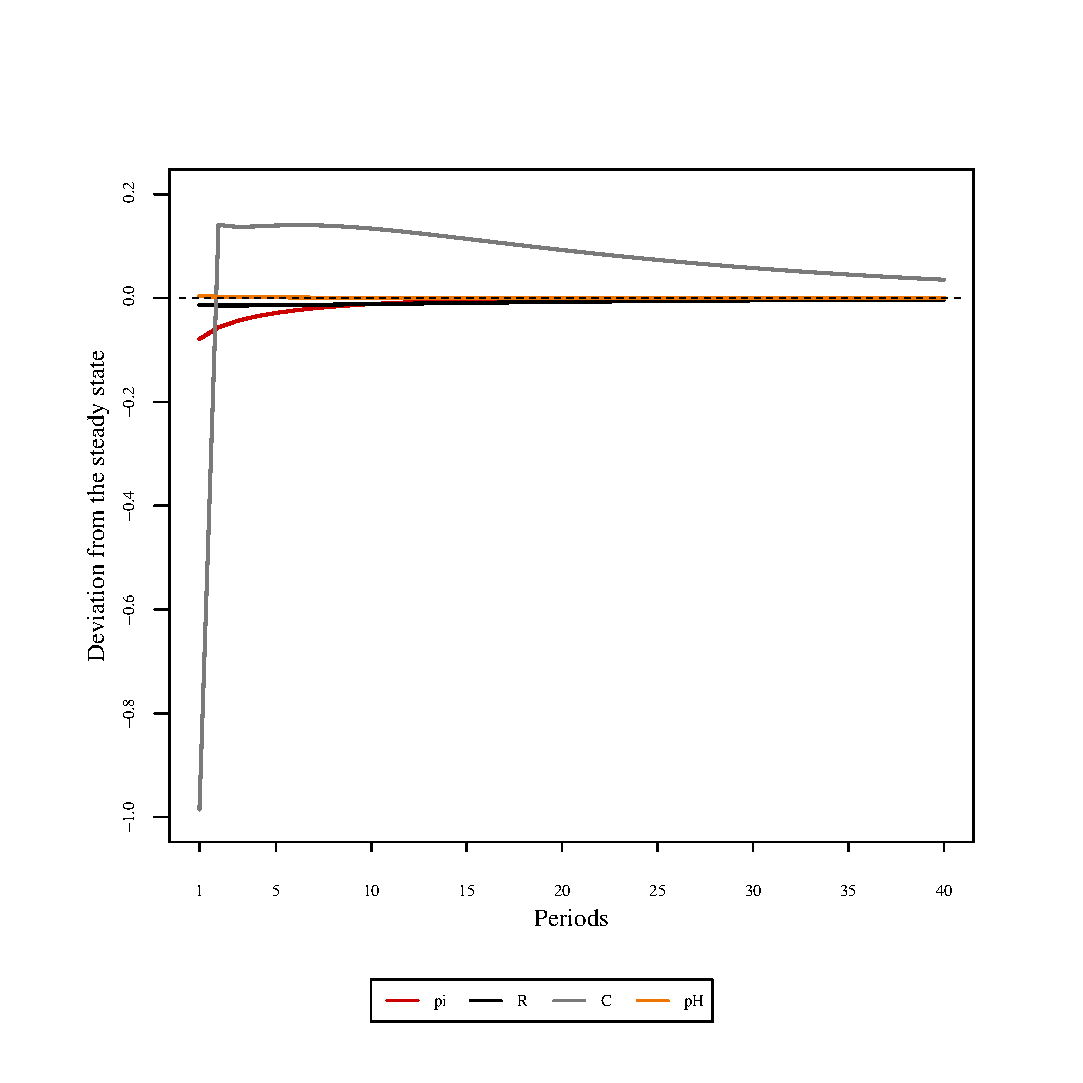
\includegraphics[width=0.99\textwidth, scale=0.55]{plots/plot_31.eps}
\caption{Impulse responses ($\pi, R, C, {p\!H}$) to $\epsilon^{\mathrm{Z}}$ shock}
\end{minipage}
\begin{minipage}{0.5\textwidth}
\vspace*{-3em}
\centering
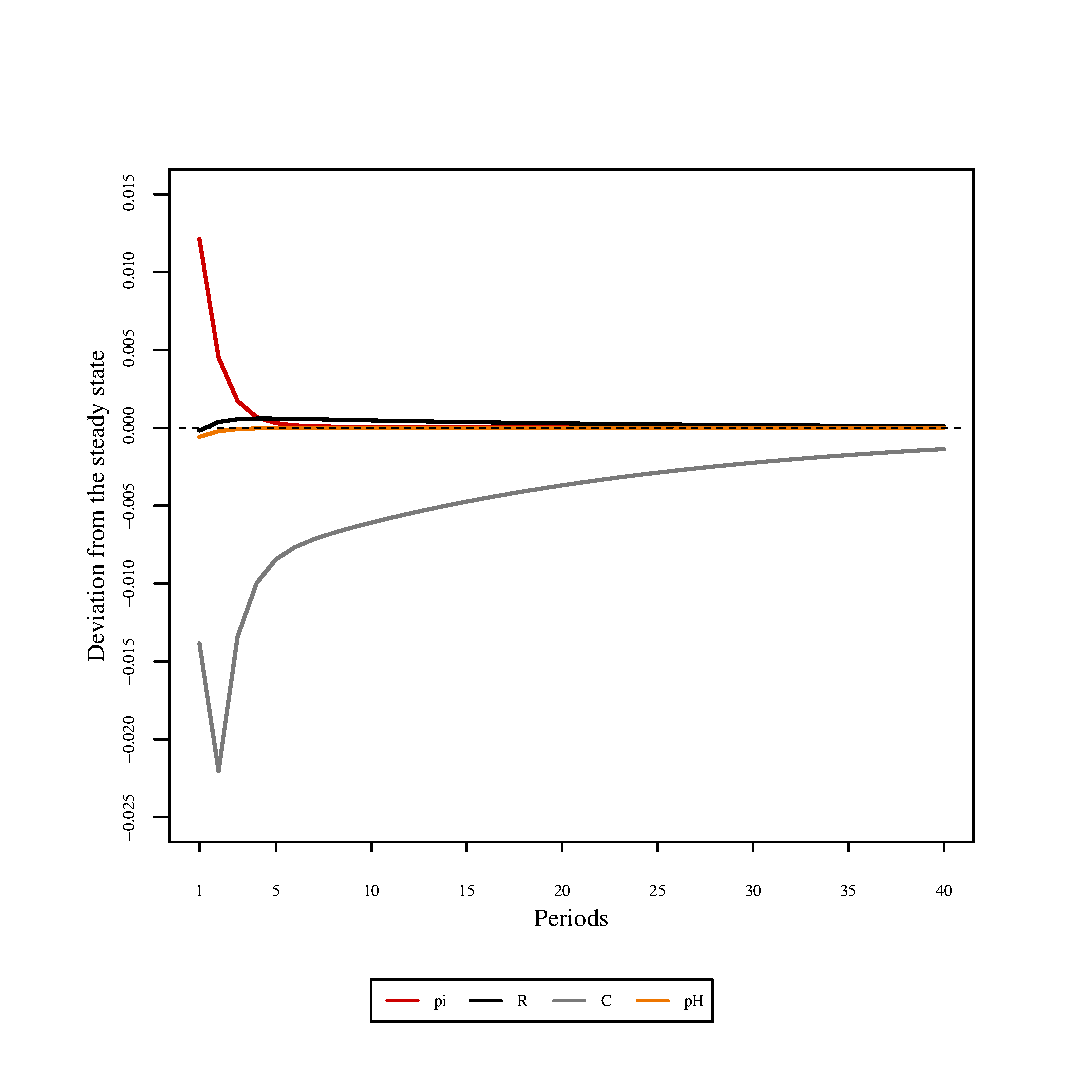
\includegraphics[width=0.99\textwidth, scale=0.55]{plots/plot_32.eps}
\caption{Impulse responses ($\pi, R, C, {p\!H}$) to $\eta^{\mathrm{p}}$ shock}
\end{minipage}
\end{figure}

\begin{figure}[h]
\begin{minipage}{0.5\textwidth}
\vspace*{-3em}
\centering
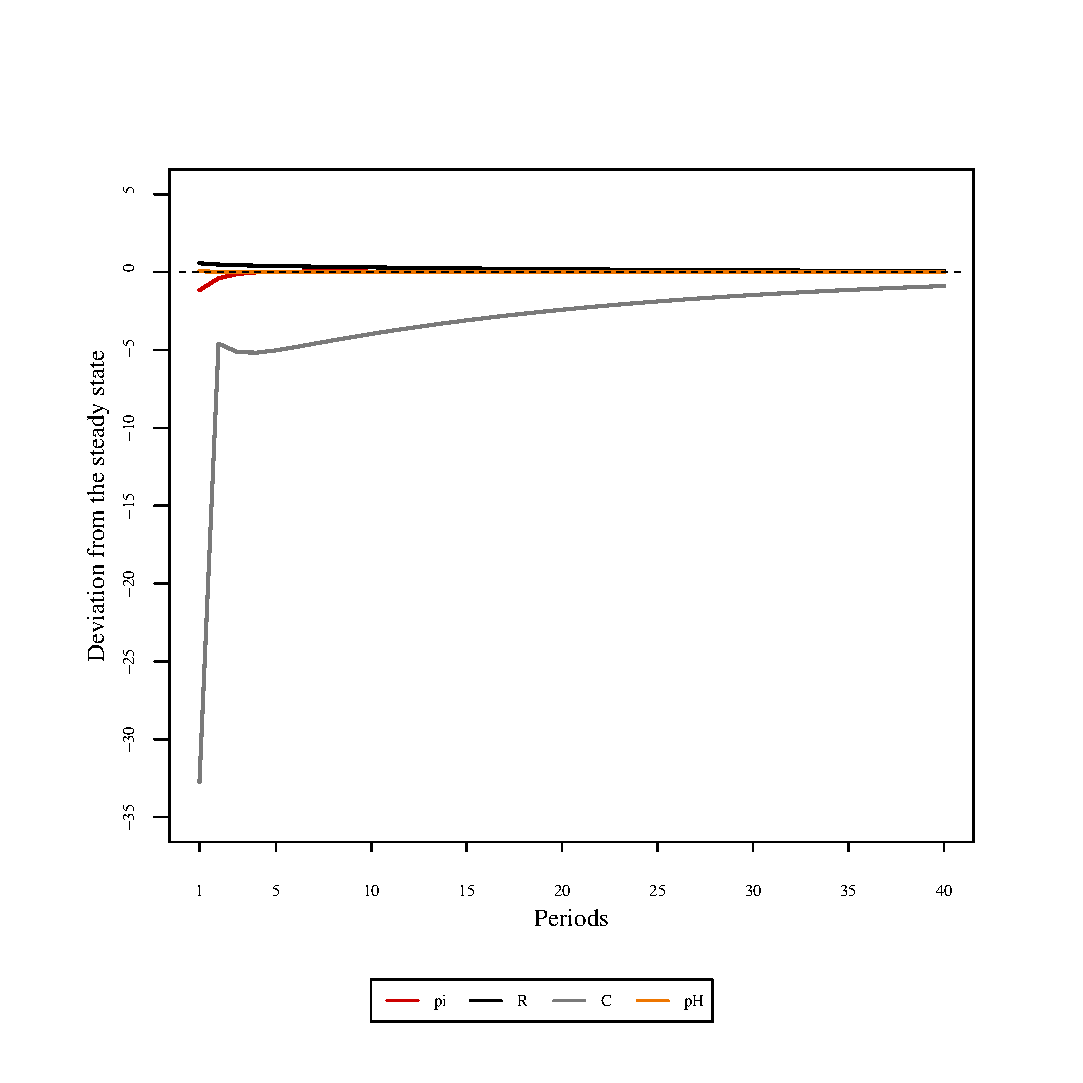
\includegraphics[width=0.99\textwidth, scale=0.55]{plots/plot_33.eps}
\caption{Impulse responses ($\pi, R, C, {p\!H}$) to $\eta^{\mathrm{R}}$ shock}
\end{minipage}
\begin{minipage}{0.5\textwidth}
\vspace*{-3em}
\centering
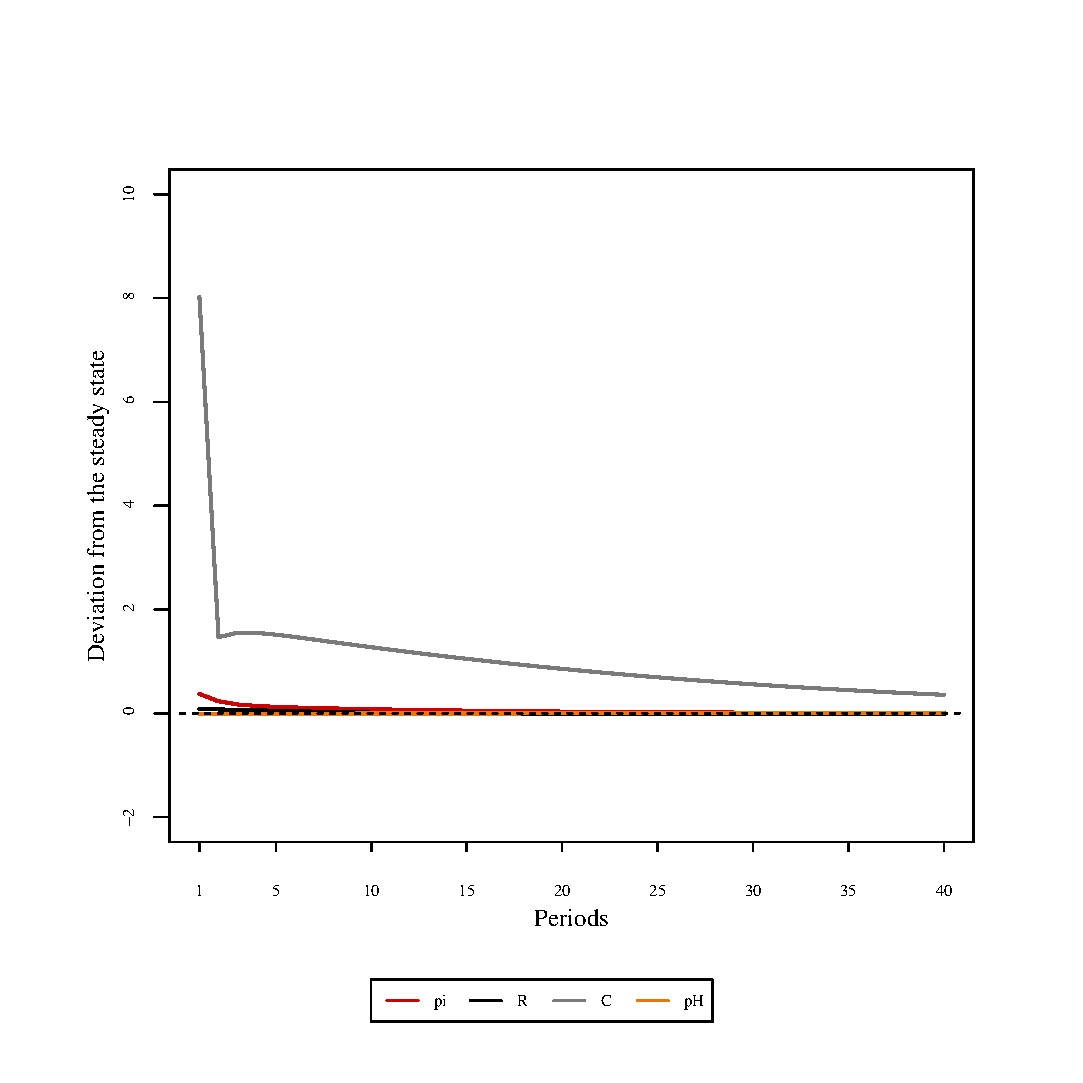
\includegraphics[width=0.99\textwidth, scale=0.55]{plots/plot_34.eps}
\caption{Impulse responses ($\pi, R, C, {p\!H}$) to $\eta^{\pi}$ shock}
\end{minipage}
\end{figure}

\pagebreak

\begin{figure}[h]
\centering
\begin{minipage}{0.5\textwidth}
\vspace*{-3em}
\centering
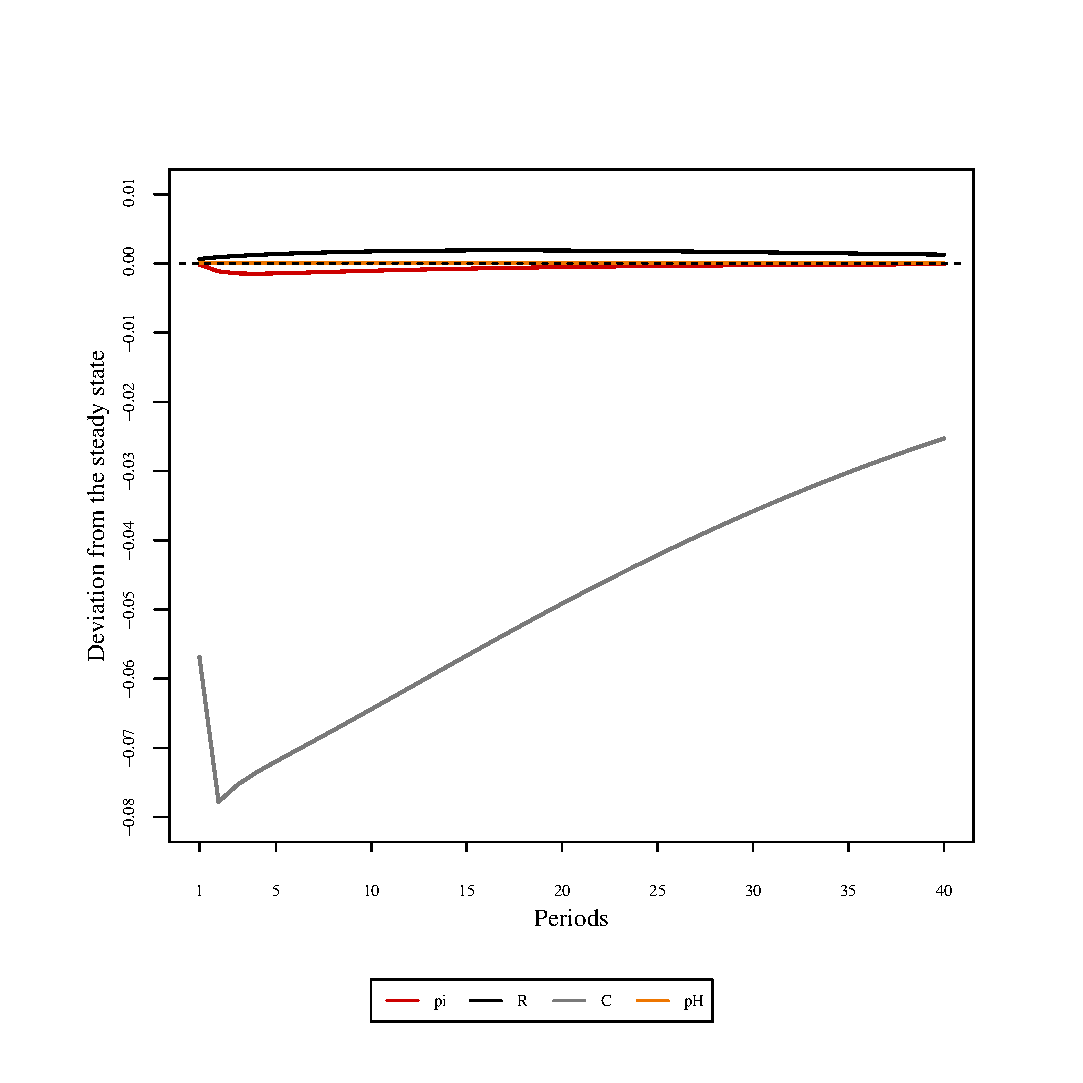
\includegraphics[width=0.99\textwidth, scale=0.55]{plots/plot_35.eps}
\caption{Impulse responses ($\pi, R, C, {p\!H}$) to $\eta^{\mathrm{G}}$ shock}
\end{minipage}
\end{figure}
